\documentclass{article}
\usepackage{graphicx}
\usepackage{hyperref}
\usepackage{caption}
\usepackage{subcaption}
\usepackage{mathtools}
\usepackage[dutch]{babel}

\begin{document}

\begin{center}
	\huge{Wiskunde in Kunst}\\
	\LARGE{Opdracht 5} \\
	
	\vspace{2cm}
	
	\Large{Fractals kunstwerken}\\
	
	\vfill
	
	\begin{figure}[Hh]
		\centering
		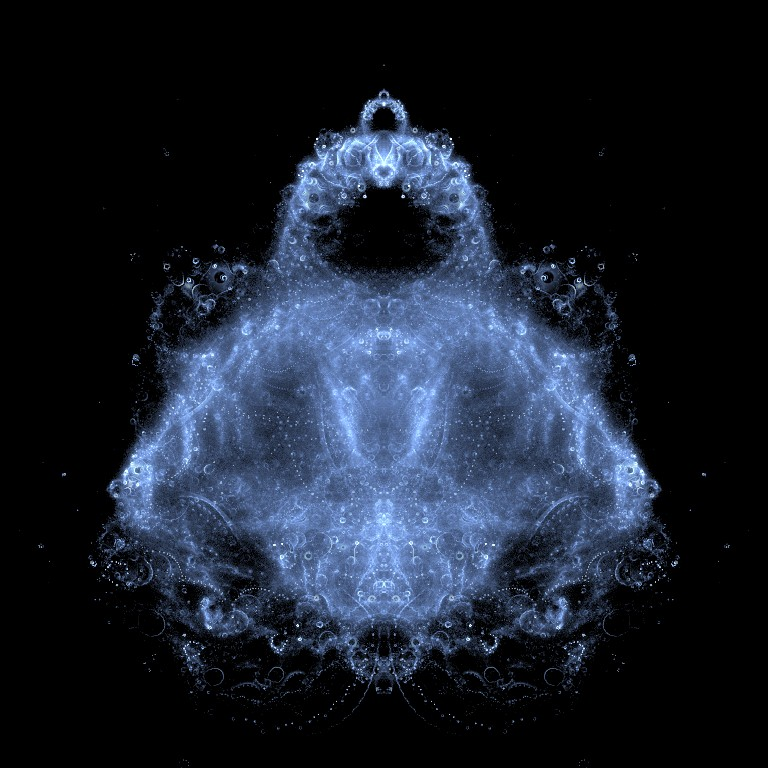
\includegraphics[width=\textwidth]{Buddhabrot-deep.jpg}
	\end{figure}
	
	\vfill
	\Large{Marcelo Dias Avelino} \hfill \large{0840416}
\end{center}

\thispagestyle{empty} % Remove page numbering

\pagebreak

\setcounter{page}{1} % Start counting pages here

\section{Overeenkomsten}

In Figuur \ref{fig:spiral-fractal} zijn twee voorbeelden van te zien van logaritmische spiralen, een soort fractal die heel vaak in de natuur voorkomt. De kunstwerk die te zien is in Figuur \ref{fig:breaking-glass} is een kunstwerk van de Nederlandse kunstenares Yvonne Mous, een kunstenares die vooral kunst creëert die gebaseerd is op fractals. De fractal in Figuur \ref{fig:logarithm-spiral} is een gedeelte van de Mandelbrot fractal.

\begin{figure}[Hh]
    \centering
    \begin{subfigure}[b]{0.48\textwidth}
        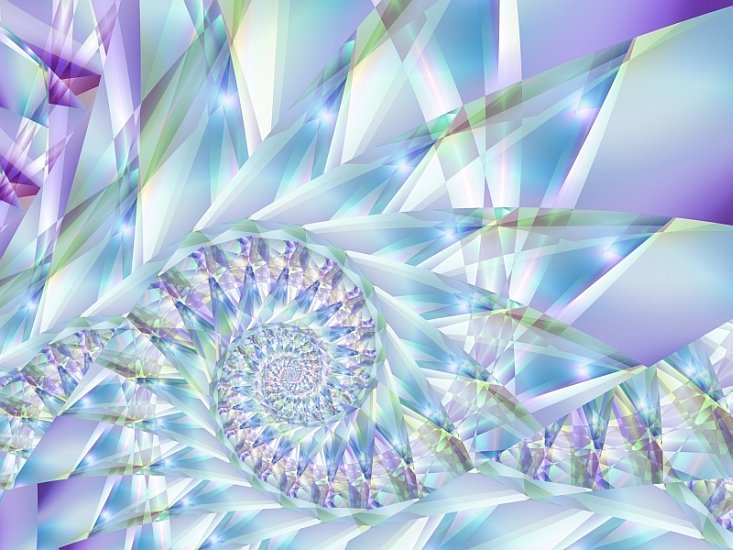
\includegraphics[width=\textwidth]{breaking-glass.jpg}
		\caption{``Breaking glass''.}
		\label{fig:breaking-glass}
    \end{subfigure}
    ~ 
    \begin{subfigure}[b]{0.48\textwidth}
        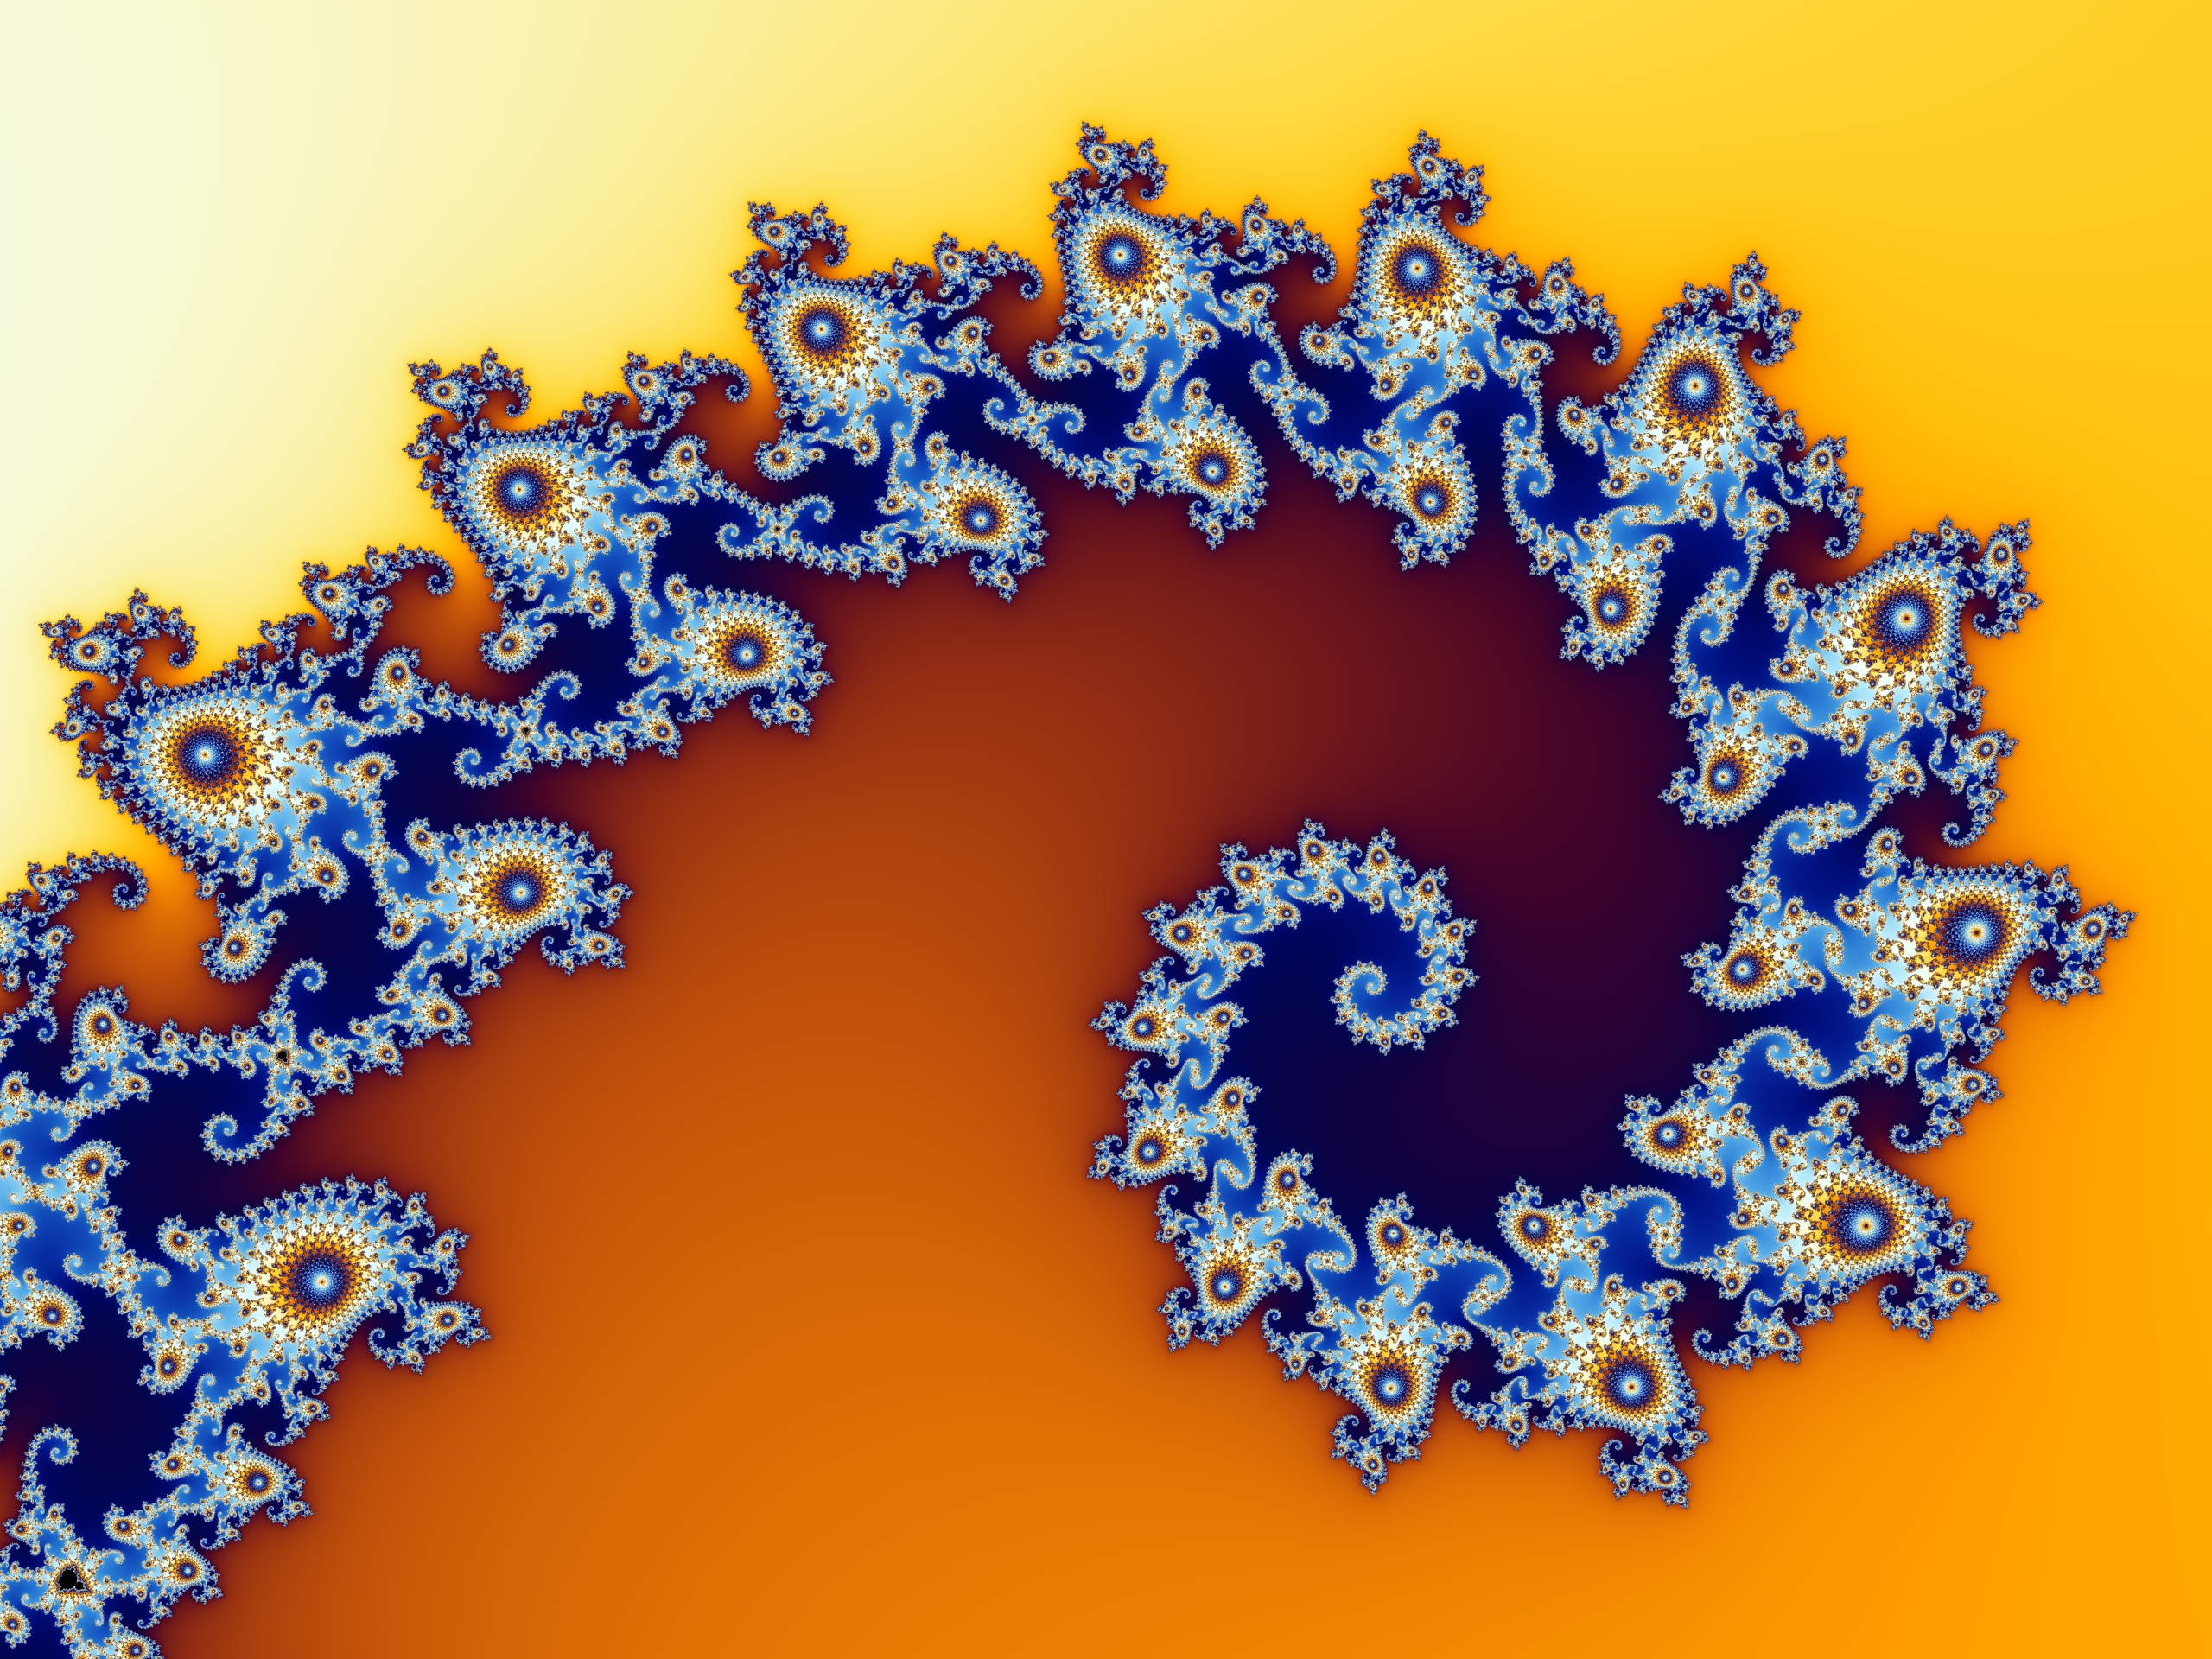
\includegraphics[width=\textwidth]{Mandel_zoom.jpg}
		\caption{Logaritmische spiraal.}
		\label{fig:logarithm-spiral}
    \end{subfigure}%
    \caption{Spiraal fractals.}
    \label{fig:spiral-fractal}
\end{figure}

De tweede voorbeeld van fractals in kunst is afgebeeld is een zogenaamd Juliaverzameling. Het is fractal gegenereerd door een functie is kenmerkend aan het feit dat bij een kleine verschil in gegeven parameters er een grote verschil ontstaat in de geproduceerd uitkomst. Een voorbeeld hiervan is te zien op Figuur \ref{fig:julia-fractal}. In de kunstwerk van Figuur \ref{fig:rolling-hills} is het duidelijk te zien de gelijkenis met de afbeelding er naast. Dit is ook een kunstwerk van Yvonne Mous.

\begin{figure}[Hh]
    \centering
    \begin{subfigure}[b]{0.48\textwidth}
        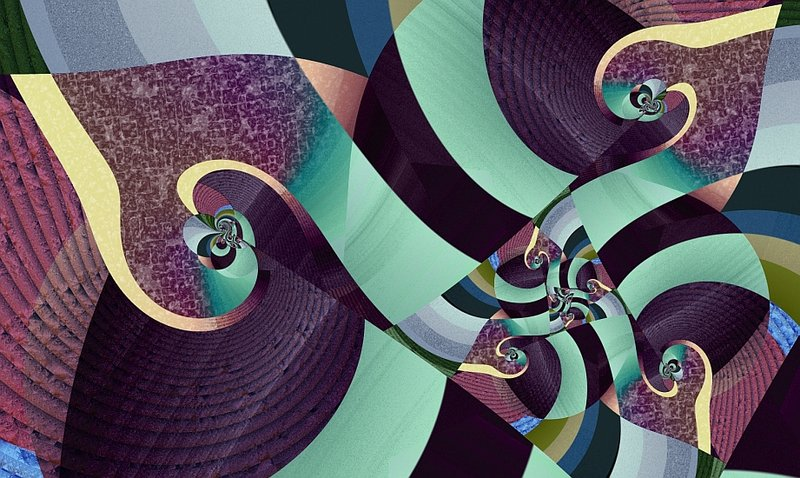
\includegraphics[width=\textwidth]{rolling-hills.jpg}
        \caption{``Rolling Hills''.}
        \label{fig:rolling-hills}
    \end{subfigure}
    ~ 
    \begin{subfigure}[b]{0.48\textwidth}
        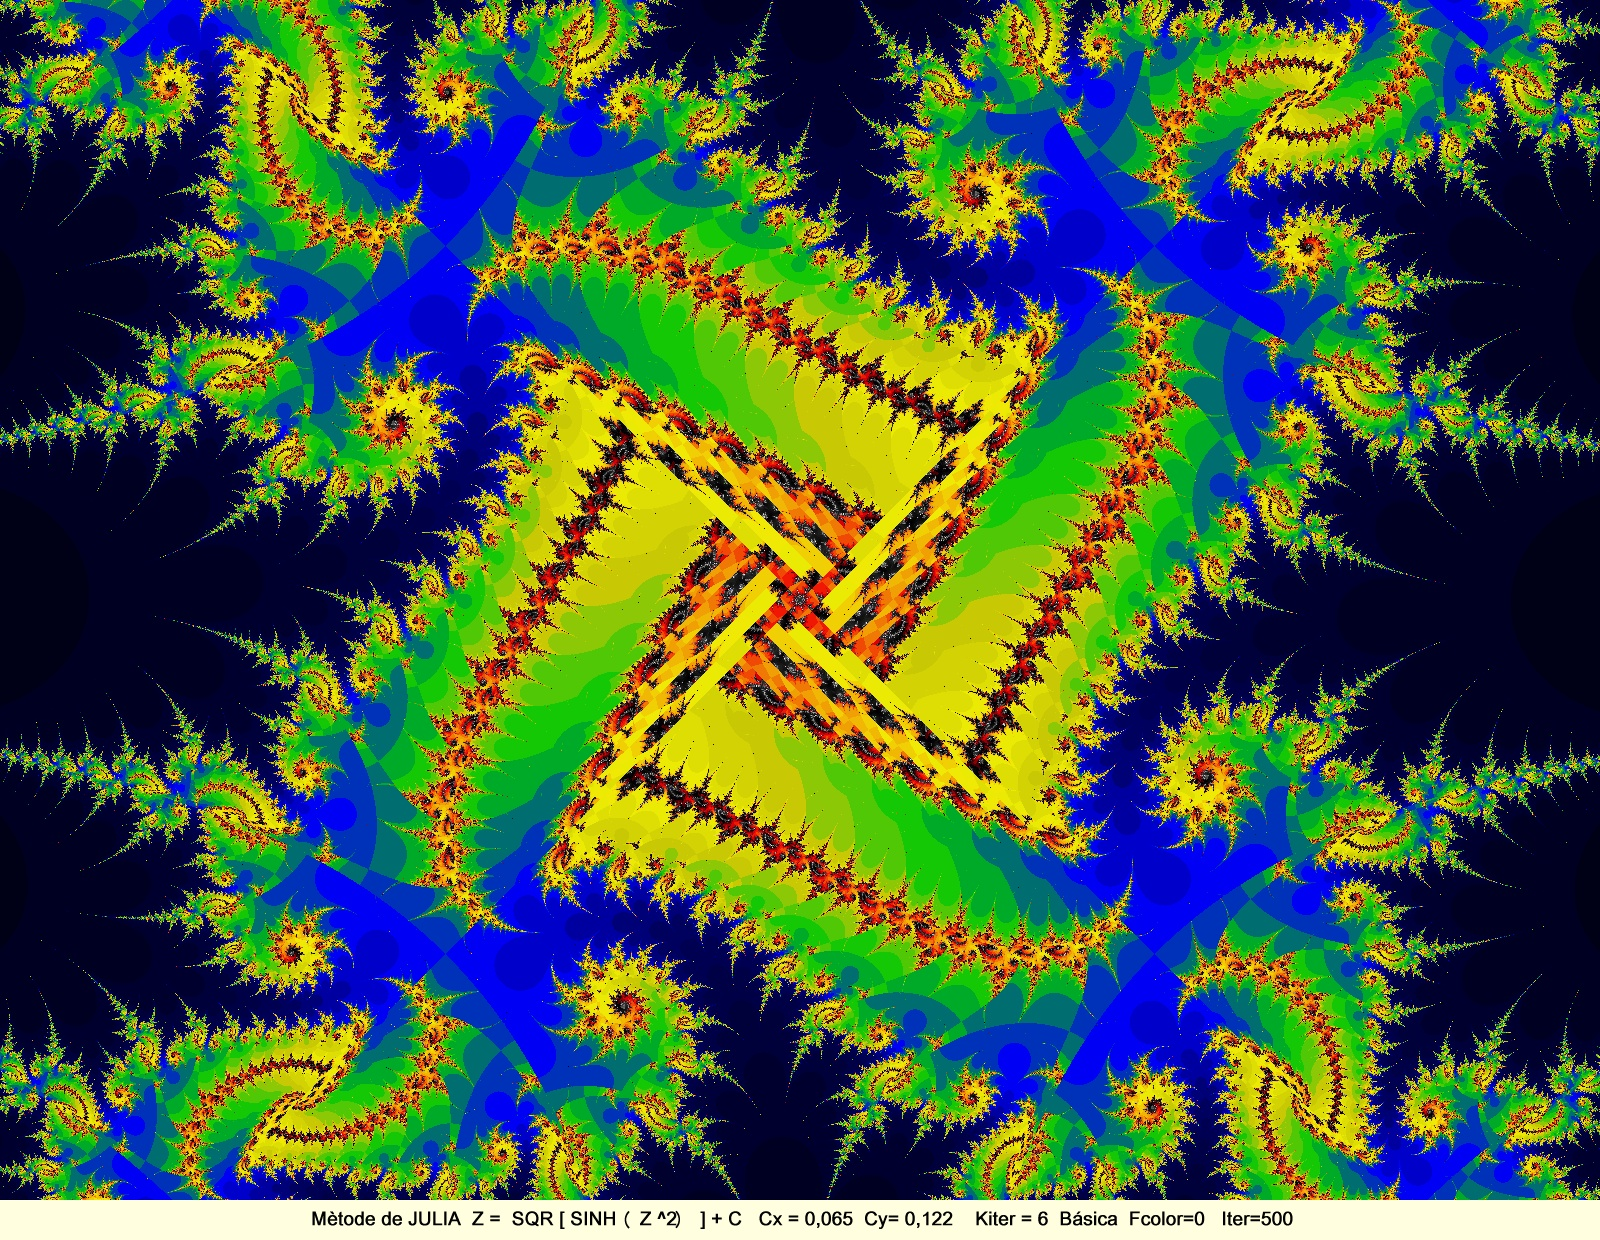
\includegraphics[width=\textwidth]{Julia-set2}
        \caption{Julia fractal.}
        \label{fig:julia-fractal}
    \end{subfigure}%
    \caption{Juliaverzameling.}
    \label{fig:julia-sets}
\end{figure}

Als laatste komen twee voorbeelden van de Heighway draak fractal en was voor het eerst onderzocht door NASA wetenschapper John Heighway. Deze soort fractal onstaat na elke segment, twee nieuwe segmenten toe te voegen op een 45 graden hoek van elkaar. In Figuur \ref{fig:veil} is een kunstwerk te zien van Kerry Mitchell, genaamd ``Veil'', dat de kenmerken van de Heighway fractal overneemt.

\begin{figure}[Hh]
    \centering
    \begin{subfigure}[b]{0.48\textwidth}
        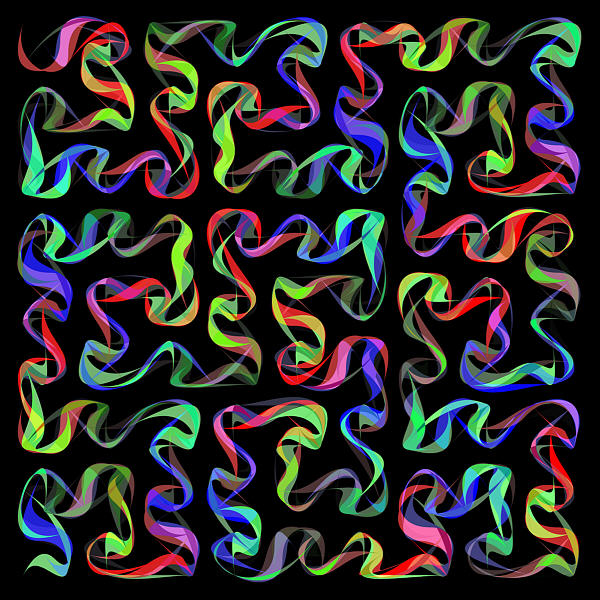
\includegraphics[width=\textwidth]{veil}
        \caption{``Veil''.}
        \label{fig:veil}
    \end{subfigure}
    ~ 
    \begin{subfigure}[b]{0.48\textwidth}
        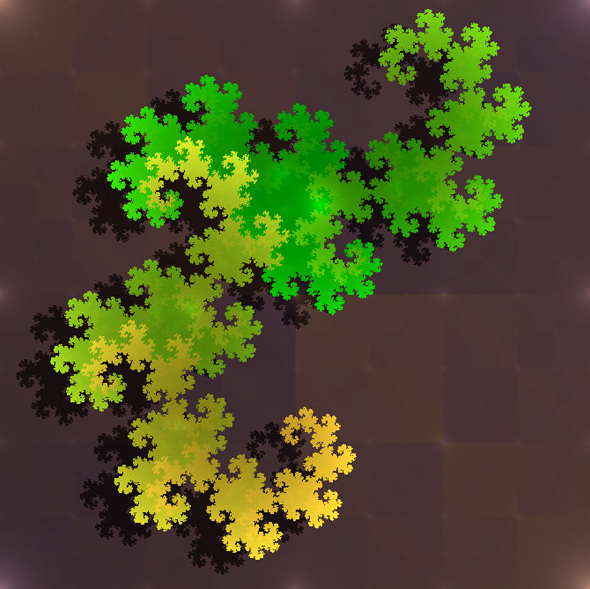
\includegraphics[width=\textwidth]{Fractal_dragon_curve}
        \caption{Boog fractal.}
        \label{fig:julia-fractal}
    \end{subfigure}%
    \caption{De draak boog.}
    \label{fig:julia-sets}
\end{figure}

\end{document}